\section{Testing}

\subsection{Testing Table}
\subsubsection{Targetted Testing Areas}

\large
As part of testing my NEA, I identified the key areas of my project which needed testing.
My testing targets these areas from different angles to ensure they work correctly. 
These areas are:
\begin{enumerate}
    \item User Input and Program Output
        \begin{enumerate}
            \item Parameter Loading
            \item Neural Network Loading
            \item Graphical Output
            \item Console Output
        \end{enumerate}
    \item Matrix Implementation
        \begin{enumerate}
            \item Constructor Cases
            \item Matrix Operations
            \item Thrown Exceptions
        \end{enumerate}
    \item Deep Q Learning Algorithm
        \begin{enumerate}
            \item Forward Propagation
            \item Loss Function
            \item Back Propagation
            \item Double Ended Queue Data Type
        \end{enumerate}
    \item Data Logger
        \begin{enumerate}
            \item Data Structure Matching
            \item Heap Data Structure
            \item Heap Sort Implementation
        \end{enumerate}
    \item Simulation
        \begin{enumerate}
            \item Generation of 2d Terrain
            \item Continuity of Generation
            \item ML Agent
            \item Reward Methods
        \end{enumerate}
\end{enumerate}

\pagebreak

\begin{center}
    \large
    \textbf{Below is included an NEA Testing video used for some parts of Testing Evidence}
    
    \vspace{0.2cm}
    
    \Large
    \textit{https://thisisalink.com/youtotallybelieveme/}
\end{center}

\vspace{1cm}
\subsubsection{User Input and Program Output Tests}
\vspace{0.5cm}

\normalsize
\begin{longtable}{| C{0.6cm} | C{3cm} | C{4cm} | C{5cm} | L{1cm} | L{1.4cm} |}
    \hline
    {\footnotesize Test No.} & Test Name & Input Data / Description & Expected Output & Pass / Fail & Testing Evidence \\
    \hline\hline
    \rn & Loading Parameters File & Input "Default.param" file which contains the loadable values & Loads parameters into the 
    Parameters Dictionary variable & Pass & 1.1 \\ 
    \hline
    \rn & Parameters within range & Input Loaded Parameters Dictionary & Prints to console "Parameters within Specified Ranges" & Pass & 1.2 \\
    \hline
    \rn & Below Range Parameter & Input "Default.param" file with a below range parameters & Raises an exception detailing the Parameter, 
    Value of Parameters, and the given Range Required & Pass & 1.3 \\
    \hline
    \rn & Above Range Parameter & Input "Default.param" file with an above range parameters & Raises an exception detailing the Parameter, 
    Value of Parameters, and the given Range Required  & Pass & 1.4 \\
    \hline
    \rn & Network Saved Data Loading & When Prompted to load network data type "Y", and type the file name of network data to load & Network 
    Data is loaded successfully, training position stored & Pass & 1.5 \\
    \hline
    \rn & Window Opening & Run Program, enter setup info as normal & Window opens and is of the correct size/resolution & Pass & 1.6 \\
    \hline
    \rn & Window Displays correct debug information & Run Program, enter setup info as normal, with "Debug" = 1 in parameters file & Debug 
    Layer output info displayed on Right side of Window & Pass & 1.7 \\
    \hline
    \rn & Agent is displayed & Run Program, enter setup info as normal & Orange square displayed on screen & Pass & 1.8 \\
    \hline
    \rn & Enemies are displayed & Run Program, enter setup info as normal, with "StartEnemyCount" $\greatereq$ 1  & Red Square/s are displayed 
    on Screen & Pass & 1.9 \\
    \hline
    \rn & Console Messages Output & Run Program, enter setup info as normal & Console Messages Outputted per 100 Steps & Pass & 1.10 \\
    \hline
\end{longtable}

\vspace{1cm}
\setcounter{magicrownumbers}{0}
\subsubsection{Matrix Implementation Tests}
\vspace{0.5cm}

\normalsize
\begin{longtable}{| C{0.6cm} | C{3cm} | C{4cm} | C{5cm} | L{1cm} | L{1.4cm} |}
    \hline
    {\footnotesize Test No.} & Test Name & Input Data / Description & Expected Output & Pass / Fail & Testing Evidence \\
    \hline\hline
    \rn & Create Matrix with Tuple & A Tuple for the order of the Matrix & Matrix is created with an order the same as the Tuple & Pass & 2.1 \\
    \hline
    \rn & Create Matrix with 2d List & A 2d List, where the parent list holds a list for every row, each "row list" is of the same length & Matrix is created with the same values as the 2d List & Pass & 2.2 \\
    \hline
    \rn & Create Vector with List & A 1d List of any Values  & Vector is created with the same values as the List & Pass & 2.3 \\
    \hline
    \rn & Print Matrix to Console & A valid Matrix of any size & Matrix Prints to the console with the correct formatting & Pass & 2.4 \\
    \hline
    \rn & Create Randomized Matrix & A Tuple for the order of the Matrix, and the keyargument random=True & Matrix is created with randomized values between -0.5 and 0.5 & Pass & 2.5 \\
    \hline
    \rn & Create Identity Matrix & A Tuple for the order of the Matrix, and the keyargument identity=True & Matrix is created with all 0's and 1's down the diagonal & Pass & 2.6 \\
    \hline
    \rn & Matrix Addition Calculation & Two Matrices of the same order & Matrix Addition is performed to create a new Matrix with the added values & Pass & 2.7 \\
    \hline
    \rn & Matrix Subtraction Calculation & Two Matrices of the same order & Matrix Subtraction is performed to create a new Matrix with the subtracted values & Pass & 2.8 \\
    \hline
    \rn & Matrix Multiplication Calculation & Two Matrices where Width of $M1$ is equal to the height of $M2$ & Matrix Multiplication is performed to create a new Matrix with the multiplied values & Pass & 2.9 \\
    \hline
    \rn & Matrix Scalar Multiplication Calculation & A $float/int$ as the scalar and any size Matrix & Matrix Scalar Multiplication is performed to create a new Matrix with the multiplied values & Pass & 2.10 \\
    \hline
    \rn & Vector Hadamard Product Calculation & Two Vectors with the same Order & Vector Hadamard Product is performed to create a new Vector with the multiplied values & Pass & 2.11 \\
    \hline
    \rn & Matrix Power Calculation & A Square Matrix with values stored in it & Matrix to the Power of is performed to create a new Matrix with the correct values & Pass & 2.12 \\
    \hline
    \rn & Matrix Transpose Calculation & A Matrix with values stored in it & New Matrix is created with values flipped across the diagonal & Pass & 2.13 \\
    \hline
    \rn & Matrix Select Column & A Matrix with values stored in it & Selects the indexed Column from the Matrix, returning as a list & Pass & 2.14 \\
    \hline
    \rn & Matrix Select Row & A Matrix with values stored in it & Selects the indexed Row from the Matrix, returning as a list & Pass & 2.15 \\
    \hline
    \rn & Vector Max in Vector & A Vector & Returns the Largest value in Vector & Pass & 2.16 \\
    \hline
    \rn & Matrix Clear & A Matrix with values stored in it & Clears Matrix of any values & Pass & 2.17 \\
    \hline
    \rn & Combine Vectors & List of Vectors of the same Order & Combines the list of Vectors into a Matrix & Pass & 2.18 \\
    \hline
    \rn & Matrix Sum & - & Sums all values in the Matrix returning a $float/int$ & Pass & 2.19 \\
    \hline
    \rn & Randomized Matrix Constructor Tests & Generator Constructor Parameters randomly for 10000 Tests & All Tests Should produce a valid Matrix & Pass & 2.16 \\
    \hline
    \rn & Randomized Constructor Exception Tests & Generate Random Data to cause Exceptions within the Constructor for 10000 Tests & All Tests should 
    trigger the Targetted Exception for that test & Pass & 2.17 \\
    \hline
    \rn & Randomized Operator Tests & Generator Random Data to test the Operator Methods for 10000 Tests & All Tests should produce the correct result & Pass & 2.18 \\
    \hline
    \rn & Randomized Operator Exception Tests & Generate Random Data to cause Exceptions within the Operators for 10000 Tests & All Tests should 
    trigger the Targetted Exception for that test & Pass & 2.19 \\
    \hline
\end{longtable}

\vspace{1cm}
\setcounter{magicrownumbers}{0}
\subsubsection{Deep Reinforcement Learning Algorithm Tests}
\vspace{0.5cm}

\small
\begin{longtable}{| C{0.6cm} | C{3cm} | C{4cm} | C{5cm} | L{1cm} | L{1.4cm} |}
\hline
{\footnotesize Test No.} & Test Name & Input Data / Description & Expected Output & Pass / Fail & Testing Evidence \\
    \hline\hline
    \rn & Networks are Created & Run Program, enter setup info, denying the loading of weights & A Dual Neural Network is created after Program Start & Pass & 3.1 \\
    \hline
    \rn & Networks conforms to Parameters & Run Program, enter setup info, denying the loading of weights & The created Dual Neural Network conforms to the specified structure 
    in the parameter "DeepQLearningLayers" & Pass & 3.2 \\
    \hline
    \rn & Forward Propagation Test & Run program as normal & Actions are predicted by the Network & Pass & 3.3 \\
    \hline
    \rn & Loss Function & Run program as normal & Loss is calculated & Pass & 3.4 \\
    \hline
    \rn & Back Propagation Test & Run program as normal & Calculated Loss is Back Propagated through the Network & Pass & 3.5 \\
    \hline
    \rn & Deque Push Front & A value to push to the Deque & Item is pushed to front of Deque & Pass & 3.6 \\
    \hline
    \rn & Deque First/Last & Call the .First() or .Last() Method for a Deque Object & Returns item at Front/Last index of Deque & Pass & 3.7 \\
    \hline
    \rn & Deque Sample N Amount of Items & Call the .Sample(int N) Method, with a parameter of N items, for a Deque Object & Returns N number of random 
    samples from Deque & Pass & 3.8 \\
    \hline
    \rn & Experience Replay Sampling & Run program as normal & Back Propagation is performed on the sampled Deque Items & Pass & 3.9 \\
    \hline
    \rn & Activation Outputs Unit Test & Input Value Vector to the Activation Function & Returns a Vector of values, where the Activation has been 
    applied to them & Pass & 3.10 \\
    \hline
    \rn & Activation Derivatives Output Unit Test & Input Value Vector to the Activation Derivative Function & Returns a Vector of values, where the 
    Activation Derivative has been applied to them & Pass & 3.11 \\
    \hline
\end{longtable}

\vspace{1cm}
\setcounter{magicrownumbers}{0}
\subsubsection{Data Logger Tests}
\vspace{0.5cm}

\normalsize
\begin{longtable}{| C{0.6cm} | C{3cm} | C{4cm} | C{5cm} | L{1cm} | L{1.4cm} |}
\hline
{\footnotesize Test No.} & Test Name & Input Data / Description & Expected Output & Pass / Fail & Testing Evidence \\
    \hline\hline
    \rn & Heap Sort Descending & A randomly generated input list & Sorts the list of items into Descending order & Pass & 4.1 \\
    \hline
    \rn & Add Point & A Data Point matching the data structure of the DataCollector & Point is added to Data Points list & Pass & 4.2 \\
    \hline
    \rn & Match Data Structure with Single & Data Structure constrains an index with a Single-Typed 
    definition & No error thrown & Pass & 4.3 \\
    \hline
    \rn & Match Data Structure with Multi-Typed & Data Structure constrains an index with a Multi-Typed
    definition & No error thrown & Pass & 4.4 \\
    \hline
    \rn & Match Data Structure with List-Typed & Data Structure constrains an index with a List-Typed 
    definition & No error thrown & Pass & 4.5 \\
    \hline
    \rn & Match Data Structure Error & Try match point with structure which does not match & Error is thrown with correct info & Pass & 4.6 \\
    \hline
    \rn & Select Query & Select from DataLogger with an Index and Search Contents & Returns a list of the selected column where the Search Contents Matches & Pass & 4.7 \\
    \hline
    \rn & Save Data Points & Invoke Save method on DataLogger Object & Saves Data Points to specified File & Pass & 4.8 \\
    \hline
    \rn & Load Data Points & Invoke Load method on DataLogger Object & Loads Data Points from specified File & Pass & 4.9 \\
    \hline
\end{longtable}

\vspace{1cm}
\setcounter{magicrownumbers}{0}
\subsubsection{Simulation Tests}
\vspace{0.5cm}

\normalsize
\begin{longtable}{| C{0.6cm} | C{3cm} | C{4cm} | C{5cm} | L{1cm} | L{1.4cm} |}
\hline
{\footnotesize Test No.} & Test Name & Input Data / Description & Expected Output & Pass / Fail & Testing Evidence \\
    \hline\hline
    \rn & Creation of Agent & Run program as normal & Agent is created as an instance of the Agent Class & Pass & 5.1 \\
    \hline
    \rn & Creation of Enemies & Run program as normal with the "StartEnemyCount" Parameter $\greatereq 1$ & Up to the amount of specified Enemies are created & Pass & 5.2 \\
    \hline
    \rn & Enemies path find towards Agent & Run program as normal with "StartEnemyCount" Parameter $\greatereq 1$ & The spawned enemies' path find towards the agent 
    using the defined pathfinding algorithm & - & - \\
    \hline
    \rn & Getting Tile Data & Call .GetTileVector(worldMap, enemyList[]) with arguments for worldMap and the list of current Enemies & Returns a Vector of the 
    surrounding tile objects & Pass & 5.4 \\
    \hline
    \rn & Convert Tile Data & Call .TileVectorPostProcess(tileVec) with argument of the result from the Test Above & Converts Tile Data into two vectors, Greyscale 
    Colour and Tile Type & Pass & 5.5 \\
    \hline
    \rn & Reward System Test & Program running as normal & Expected reward is given to agent & Pass & 5.6 \\
    \hline
    \rn & World Generates to an Acceptable Standard & Run program as normal & Generates 2d Terrain which roughly looks realistic & Pass & 5.7 \\
    \hline
    \rn & World Generation Conforms to Parameters & Utilise inputted parameters to identify the effect they have on the world Generation & Terrain changes depending on inputting Parameters & Pass & 5.8 \\
    \hline
    \rn & Perlin Noise retains Continuity & Generate two worlds with the same seed & Perlin Noise returns same value when using the same seed twice & Pass & 5.9 \\
    \hline
\end{longtable}

\pagebreak
\vspace{1cm}
\subsection{Testing Evidence}
\vspace{0.5cm}

\subsubsection{User Input and Program Output Evidence}

\setcounter{magicrownumbers}{0}
\normalsize
\begin{center}
    {\large Evidence 1.\rn }\\ 
    \vspace{0.3cm}
    The .json file which is being loaded \\
    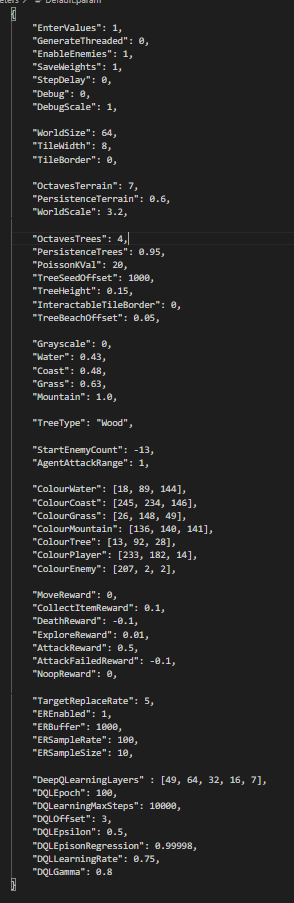
\includegraphics[width=6cm]{Images/Testing/T1.1.1.PNG} \\
    Printing the loaded Json File to Console to check the values match\\
    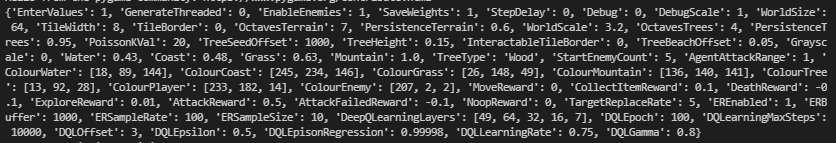
\includegraphics[width=16cm]{Images/Testing/T1.1.2.PNG} \\
    \vspace{1cm}

    {\large Evidence 1.\rn } \\ 
    \vspace{0.3cm}
    Console Output when parameters are within specified ranges \\
    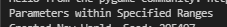
\includegraphics[width=6cm]{Images/Testing/T1.2.1.PNG} \\
    A Screenshot of the .json file where the Ranges are defined \\
    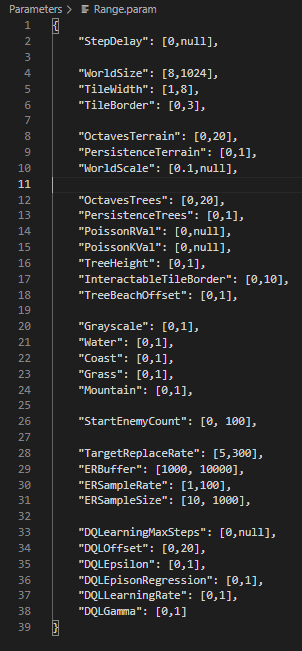
\includegraphics[width=6cm]{Images/Testing/T1.2.2.PNG}
    \vspace{1cm}

    {\large Evidence 1.\rn } \\ 
    \vspace{0.3cm}
    The given out of range parameter - subceeding \\
    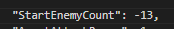
\includegraphics[width=6cm]{Images/Testing/T1.3.1.PNG} \\
    The specified range it should be within \\
    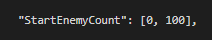
\includegraphics[width=6cm]{Images/Testing/T1.3.2.PNG} \\
    The Exception thrown when the program is run \\
    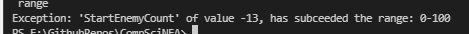
\includegraphics[width=12cm]{Images/Testing/T1.3.3.PNG} \\
    \vspace{1cm}

    {\large Evidence 1.\rn }\\ 
    \vspace{0.3cm}
    The given out of range parameter - exceeding \\
    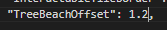
\includegraphics[width=6cm]{Images/Testing/T1.4.1.PNG} \\
    The specified range it should be within \\
    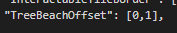
\includegraphics[width=6cm]{Images/Testing/T1.4.2.PNG} \\
    The Exception thrown when the program is run \\
    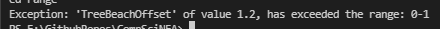
\includegraphics[width=12cm]{Images/Testing/T1.4.3.PNG} \\
    \vspace{1cm}

    {\large Evidence 1.\rn }\\ 
    \vspace{0.3cm}
    The Console prompt if the user wants to load Network Weights \\
    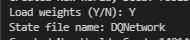
\includegraphics[width=6cm]{Images/Testing/T1.5.1.PNG} \\
    The file the program is loading \\
    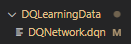
\includegraphics[width=4cm]{Images/Testing/T1.5.2.PNG} \\
    The testing step resumes at 400, underlined in Red \\
    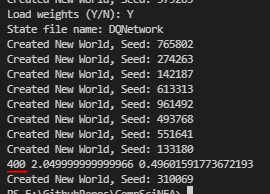
\includegraphics[width=6cm]{Images/Testing/T1.5.3.PNG}
    \vspace{1cm}

    {\large Evidence 1.\rn } \\ 
    \vspace{0.3cm}
    The width/height of the window\\
    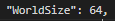
\includegraphics[width=4cm]{Images/Testing/T1.6.1.PNG} \\
    The opened window, it is 64 wide and 64 tall \\
    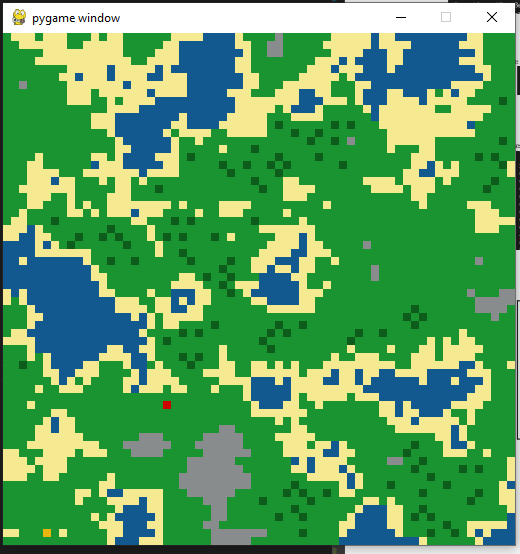
\includegraphics[width=8cm]{Images/Testing/T1.6.2.PNG}
    \vspace{1cm}

    {\large Evidence 1.\rn } \\ 
    \vspace{0.3cm}
    Debug being set to 1 in the parameters file \\
    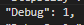
\includegraphics[width=4cm]{Images/Testing/T1.7.1.PNG} \\
    The displayed debug information to the right of the Window \\
    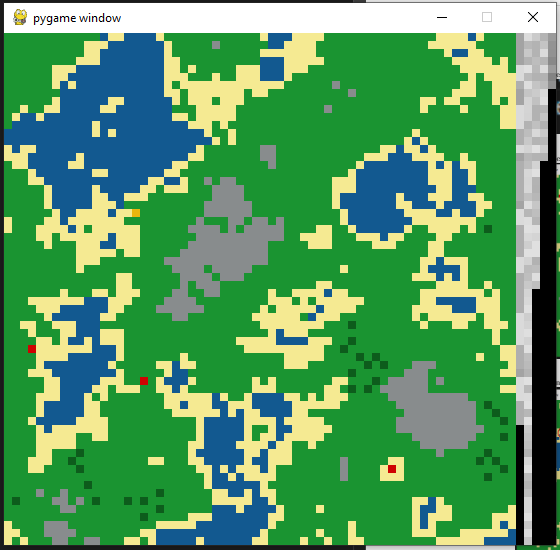
\includegraphics[width=8cm]{Images/Testing/T1.7.2.PNG} \\
    \vspace{1cm}

    {\large Evidence 1.\rn } \\ 
    \vspace{0.3cm}
    The opened window, with the agent circled \\
    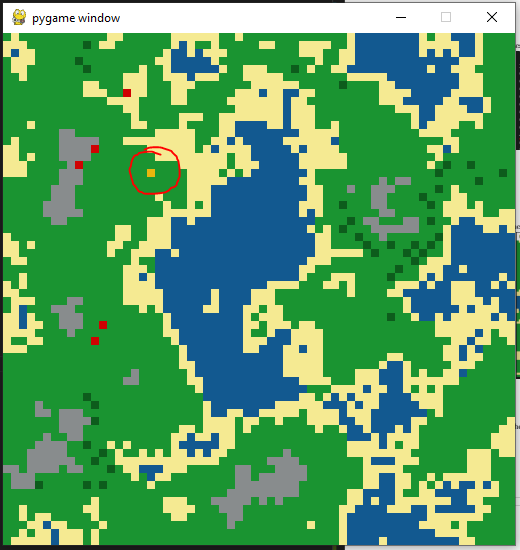
\includegraphics[width=8cm]{Images/Testing/T1.8.1.PNG} \\
    \vspace{1cm}

    {\large Evidence 1.\rn } \\ 
    \vspace{0.3cm}
    The opened window, with the enemies circled \\
    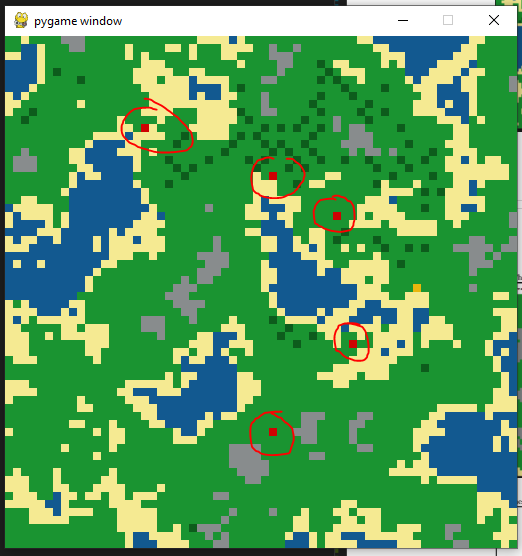
\includegraphics[width=8cm]{Images/Testing/T1.9.1.PNG} \\
    \vspace{1cm}

    {\large Evidence 1.\rn } \\ 
    \vspace{0.3cm}
    The correctly displayed console outputs \\
    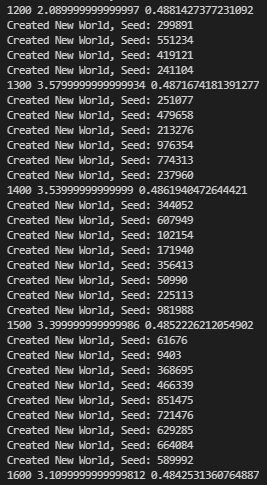
\includegraphics[width=8cm]{Images/Testing/T1.10.1.PNG} \\
\end{center}

\subsubsection{Matrix Implementation Tests}

\setcounter{magicrownumbers}{0}
\begin{center}
    {\large Evidence 2.\rn } \\ 
    \vspace{0.3cm}
    Creating a Matrix with a Tuple \\
    \begin{pythoncode}
matrix = Matrix((3, 4))
print(matrix)
    \end{pythoncode}
    The output of the above code: \\
    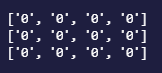
\includegraphics[width=3cm]{Images/Testing/T2.1.1.PNG} \\
    \vspace{1cm}

    {\large Evidence 2.\rn } \\ 
    \vspace{0.3cm}
    Creating a Matrix with a 2d List \\
    \begin{pythoncode}
values = [[3, 4],
        [1, 2]]
matrix = Matrix(values)
print(matrix)
    \end{pythoncode}
    The output of the above code: \\
    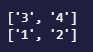
\includegraphics[width=3cm]{Images/Testing/T2.2.1.PNG} \\
    \vspace{1cm}

    {\large Evidence 2.\rn } \\ 
    \vspace{0.3cm}
    Creating a Matrix with a 1d List \\
    \begin{pythoncode}
values = [1, 2, 3, 4]
matrix = Matrix(values)
print(matrix)
    \end{pythoncode}
    The output of the above code: \\
    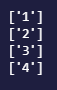
\includegraphics[width=1.5cm]{Images/Testing/T2.3.1.PNG} \\
    \vspace{1cm}

    {\large Evidence 2.\rn } \\ 
    \vspace{0.3cm}
    Printing a Matrix to the console \\
    \begin{pythoncode}
values = [[4, 3],
        [2, 1]]
matrix = Matrix(values)
print(matrix)
    \end{pythoncode}
    The output of the above code: \\
    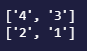
\includegraphics[width=3cm]{Images/Testing/T2.4.1.PNG} \\
    \vspace{1cm}

    {\large Evidence 2.\rn } \\ 
    \vspace{0.3cm}
    Creating a Randomised Matrix \\
    \begin{pythoncode}
matrix = Matrix((2, 2), random=True)
print(matrix)
    \end{pythoncode}
    The output of the above code: \\
    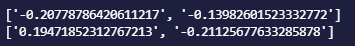
\includegraphics[width=8cm]{Images/Testing/T2.5.1.PNG} \\
    \vspace{1cm}

    {\large Evidence 2.\rn } \\ 
    \vspace{0.3cm}
    Creating an Identity Matrix \\
    \begin{pythoncode}
matrix = Matrix((3, 3), identity=True)
print(matrix)
    \end{pythoncode}
    The output of the above code: \\
    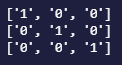
\includegraphics[width=4cm]{Images/Testing/T2.6.1.PNG} \\
    \vspace{1cm}

    {\large Evidence 2.\rn } \\ 
    \vspace{0.3cm}
    Matrix Addition Calculation \\
    \begin{pythoncode}
values = [[4, 3],
        [2, 1]]
matrix = Matrix(values)
values2 = [[3, 4],
    [1, 2]]
matrix2 = Matrix(values2)

result = matrix + matrix2
print(result)
    \end{pythoncode}
    The output of the above code: \\
    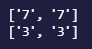
\includegraphics[width=3cm]{Images/Testing/T2.7.1.PNG} \\
    \vspace{1cm}

    {\large Evidence 2.\rn } \\ 
    \vspace{0.3cm}
    Matrix Subtraction Calculation \\
    \begin{pythoncode}
values = [[4, 3],
        [2, 1]]
matrix = Matrix(values)
values2 = [[3, 4],
    [1, 2]]
matrix2 = Matrix(values2)

result = matrix - matrix2
print(result)  
    \end{pythoncode}
    The output of the above code: \\
    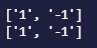
\includegraphics[width=3cm]{Images/Testing/T2.8.1.PNG} \\
    \vspace{1cm}

    {\large Evidence 2.\rn } \\ 
    \vspace{0.3cm}
    Matrix Multiplication Calculation \\
    \begin{pythoncode}
values = [[4, 3],
        [2, 1]]
matrix = Matrix(values)
values2 = [[3, 4],
        [1, 2]]
matrix2 = Matrix(values2)

result = matrix * matrix2
print(result)
    \end{pythoncode}
    The output of the above code: \\
    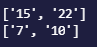
\includegraphics[width=3cm]{Images/Testing/T2.9.1.PNG} \\
    \vspace{1cm}

    {\large Evidence 2.\rn } \\ 
    \vspace{0.3cm}
    Matrix Scalar Multiplication Calculation \\
    \begin{pythoncode}
values = [[4, 3],
        [2, 1]]
matrix = Matrix(values)

result = matrix * 3 
print(result)
    \end{pythoncode}
    The output of the above code: \\
    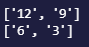
\includegraphics[width=3cm]{Images/Testing/T2.10.1.PNG} \\
    \vspace{1cm}

    {\large Evidence 2.\rn } \\ 
    \vspace{0.3cm}
    Vector Hadamard Product Calculation \\
    \begin{pythoncode}
values = [1, 2, 3, 4]
vector = Matrix(values)

values = [4, 3, 2, 1]
vector2 = Matrix(values)

result = vector * vector2
print(result)
    \end{pythoncode}
    The output of the above code: \\
    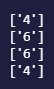
\includegraphics[width=1.5cm]{Images/Testing/T2.11.1.PNG} \\
    \vspace{1cm}

    {\large Evidence 2.\rn } \\ 
    \vspace{0.3cm}
    Matrix Power Calculation \\
    \begin{pythoncode}
values = [[4, 3],
        [2, 1]]
matrix = Matrix(values)

result = matrix ** 5
print(result)
    \end{pythoncode}
    The output of the above code: \\
    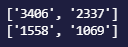
\includegraphics[width=3cm]{Images/Testing/T2.12.1.PNG} \\
    \vspace{1cm}

    {\large Evidence 2.\rn } \\ 
    \vspace{0.3cm}
    Matrix Transpose Calculation \\
    \begin{pythoncode}
values = [[4, 3],
        [2, 1]]
matrix = Matrix(values)

result = matrix.Transpose()
print(result)

    \end{pythoncode}
    The output of the above code: \\
    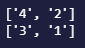
\includegraphics[width=3cm]{Images/Testing/T2.13.1.PNG} \\
    \vspace{1cm}

    {\large Evidence 2.\rn } \\ 
    \vspace{0.3cm}
    Matrix Select Column \\
    \begin{pythoncode}
values = [[4, 3, 6],
        [2, 1, 5]]
matrix = Matrix(values)

result = matrix.SelectColumn(1)
print(result)
    \end{pythoncode}
    The output of the above code: \\
    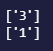
\includegraphics[width=1.5cm]{Images/Testing/T2.14.1.PNG} \\
    \vspace{1cm}

    {\large Evidence 2.\rn } \\ 
    \vspace{0.3cm}
    Matrix Select Row \\
    \begin{pythoncode}
values = [[4, 3, 6],
        [2, 1, 5]]
matrix = Matrix(values)

result = matrix.SelectRow(0)
print(result)
    \end{pythoncode}
    The output of the above code: \\
    
\includegraphics[width=3cm]{Images/Testing/T2.15.1.PNG} \\
    \vspace{1cm}
    
    {\large Evidence 2.\rn } \\ 
    \vspace{0.3cm}
    Vector Max \\
    \begin{pythoncode}
values = [4, 3, 6, 1, 2, 5]
vector = Matrix(values)

result = vector.MaxInVector()
print(result)
    \end{pythoncode}
    The output of the above code: \\
    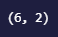
\includegraphics[width=1.5cm]{Images/Testing/T2.16.1.PNG} \\
    \vspace{1cm}
    
    {\large Evidence 2.\rn } \\ 
    \vspace{0.3cm}
    Matrix Clear \\
    \begin{pythoncode}
values = [[4, 3, 6],
        [2, 1, 5]]
matrix = Matrix(values)

matrix.Clear()
print(matrix)
    \end{pythoncode}
    The output of the above code: \\
    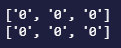
\includegraphics[width=4cm]{Images/Testing/T2.17.1.PNG} \\
    \vspace{1cm}
    
    {\large Evidence 2.\rn } \\ 
    \vspace{0.3cm}
    Matrix Combine Vectors \\
    \begin{pythoncode}
values = [1, 2, 3, 4]
vector = Matrix(values)

values = [4, 3, 2, 1]
vector2 = Matrix(values)

vectorList = [vector, vector2]

result = Matrix.CombineVectorsHor(vectorList)
print(result)
    \end{pythoncode}
    The output of the above code: \\
    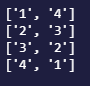
\includegraphics[width=3cm]{Images/Testing/T2.18.1.PNG} \\
    \vspace{1cm}
    
    {\large Evidence 2.\rn } \\ 
    \vspace{0.3cm}
    Matrix Sum \\
    \begin{pythoncode}
values = [[4, 3, 6],
        [2, 1, 5]]
matrix = Matrix(values)

result = matrix.Sum()
print(result)
    \end{pythoncode}
    The output of the above code: \\
    
\includegraphics[width=1.5cm]{Images/Testing/T2.19.1.PNG} \\
    \vspace{1cm}
    
    {\large Evidence 2.\rn } \\ 
    \vspace{0.3cm}
    Console Output, all Tests have passed with no failures \\
    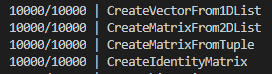
\includegraphics[width=6cm]{Images/Testing/T2.20.1.PNG} \\
    \vspace{1cm}

    {\large Evidence 2.\rn } \\ 
    \vspace{0.3cm}
    Console Output, all Tests have passed with no failures \\
    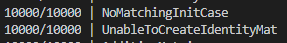
\includegraphics[width=6cm]{Images/Testing/T2.21.1.PNG} \\
    \vspace{1cm}

    {\large Evidence 2.\rn } \\ 
    \vspace{0.3cm}
    Console Output, all Tests have passed with no failures \\
    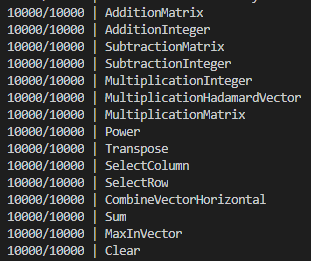
\includegraphics[width=6cm]{Images/Testing/T2.22.1.PNG} \\
    \vspace{1cm}

    {\large Evidence 2.\rn } \\ 
    \vspace{0.3cm}
    Console Output, all Tests have passed with no failures \\
    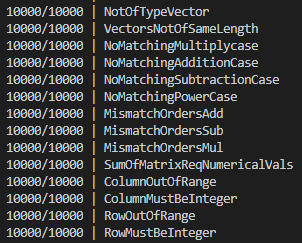
\includegraphics[width=6cm]{Images/Testing/T2.23.1.PNG} \\
    \vspace{1cm}
\end{center}

\subsubsection{Deep Q Learning Algorithm Evidence}

\setcounter{magicrownumbers}{0}
\begin{center}
    {\large Evidence 3.\rn } \\ 
    \vspace{0.3cm}
    The Neural Network objects in Memory
    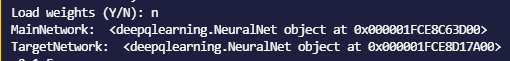
\includegraphics{Images/Testing/T3.1.1.PNG}
    \vspace{1cm}
    
    {\large Evidence 3.\rn } \\ 
    \vspace{0.3cm}
    The layer sizes upon creating the Networks \\
    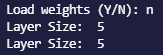
\includegraphics{Images/Testing/T3.2.1.PNG} \\
    The list of layer sizes in the parameters file \\
    
\includegraphics{Images/Testing/T3.2.2.PNG}
    \vspace{1cm}

    {\large Evidence 3.\rn } \\ 
    \vspace{0.3cm}
    Actions being printed to console, predicted by the Network \\
    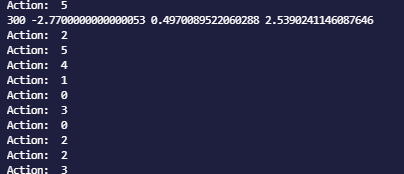
\includegraphics{Images/Testing/T3.3.1.PNG}
    \vspace{1cm}

    {\large Evidence 3.\rn } \\ 
    \vspace{0.3cm}
    Loss Vector printed to console \\
    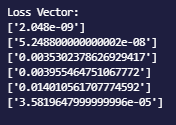
\includegraphics{Images/Testing/T3.9.2.PNG}
    \vspace{1cm}

    {\large Evidence 3.\rn } \\ 
    \vspace{0.3cm}
    Average Loss Per Step negatively declines meaning the Back Propagation is Functional \\
    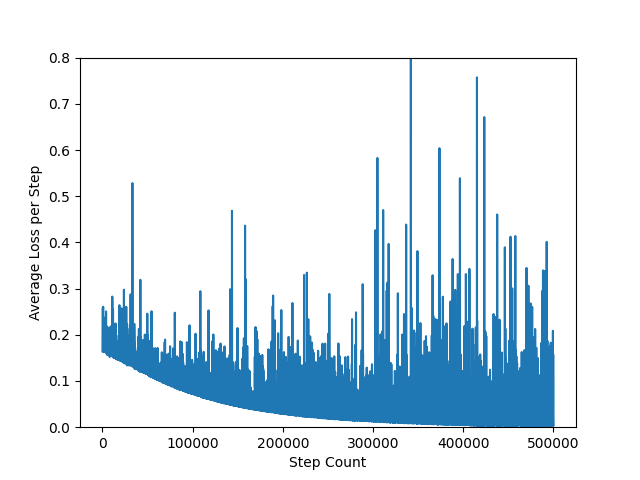
\includegraphics[width=12cm]{Images/Evaluation/RedWaterStaticExtra.png}
    \vspace{1cm}
    

    {\large Evidence 3.\rn } \\ 
    \vspace{0.3cm}
    Pushing items to the front of the Double Ended Queue \\

    \begin{pythoncode}
deque = Deque(10)
deque.PushFront(3)
print("Added 3:", deque.queue)
deque.PushFront(-5)
print("Added -1:", deque.queue)
deque.PushFront(9)
print("Added 9:", deque.queue)
    \end{pythoncode}
    
    The output of the above code: \\
    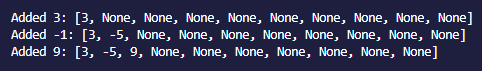
\includegraphics{Images/Testing/T3.8.1.PNG}
    \vspace{1cm}

    {\large Evidence 3.\rn } \\ 
    \vspace{0.3cm}
    Creating a Double Ended Queue with a length of 4, add Push Items to it, and get the 
    Items in First and Last \\

    \begin{pythoncode}
deque = Deque(4)
deque.PushFront(3)
deque.PushFront(-5)
deque.PushFront(9)
deque.PushFront(4)
deque.PushFront(-4)

print("First:", deque.First())
print("Last:", deque.Last())
print("Queue:", deque.queue)
    \end{pythoncode}

    The output of the above code: \\
    \includegraphics{Images/Testing/T3.9.1.PNG}
    \vspace{1cm}

    {\large Evidence 3.\rn } \\ 
    \vspace{0.3cm}
    Create a Double Ended Queue and Sample items from the Queue \\

    \begin{pythoncode}
deque = Deque(4)
deque.PushFront(3)
deque.PushFront(-5)
deque.PushFront(9)
deque.PushFront(4)
deque.PushFront(-4)

print("Sample 1:", deque.Sample(2))
print("Sample 2:", deque.Sample(2))
print(deque.queue)
    \end{pythoncode}

    The output of the above code: \\
    \includegraphics{Images/Testing/T3.10.1.PNG}
    \vspace{1cm}

    {\large Evidence 3.\rn } \\ 
    \vspace{0.3cm}
    Experience Replay buffer being sampled every 100 Steps \\
    \includegraphics{Images/Testing/T3.9.3.PNG} \\
    The parameters in Parameters file \\
    \includegraphics{Images/Testing/T3.9.4.PNG}
    \vspace{1cm}

    {\large Evidence 3.\rn } \\ 
    \vspace{0.3cm}
    Testing the Implemented Activations with specific values \\
    
    \begin{pythoncode}
outputVector = Matrix([-1, 0, 1])

Sigmoid = Sigmoid()
print("Sigmoid:")
print(Sigmoid.Activation(outputVector))

TanH = TanH()
print("TanH:")
print(TanH.Activation(outputVector))

ReLu = ReLu()
print("ReLu:")
print(ReLu.Activation(outputVector)) 

LeakyReLu = LeakyReLu()
print("LeakyReLu:")
print(LeakyReLu.Activation(outputVector))
    \end{pythoncode}

    The output of the above code: \\
    \includegraphics[width=3cm]{Images/Testing/T3.All.PNG} \\

    The WolframAlpha Sigmoid Results: \\
    \begin{figure}[H]
        \centering
        \subfloat{\includegraphics[width=4cm]{Images/Testing/T3Sigmoid-1.PNG}}
        \qquad
        \subfloat{\includegraphics[width=3cm]{Images/Testing/T3Sigmoid0.PNG}}
        \qquad
        \subfloat{\includegraphics[width=2.7cm]{Images/Testing/T3Sigmoid1.PNG}}
    \end{figure}
    

    The WolframAlpha TanH Results: \\
    \begin{figure}[H]
        \centering
        \subfloat{\includegraphics[width=3.2cm]{Images/Testing/T3Tanh-1.PNG}}
        \qquad
        \subfloat{\includegraphics[width=3cm]{Images/Testing/T3Tanh0.PNG}}
        \qquad
        \subfloat{\includegraphics[width=3.8cm]{Images/Testing/T3Tanh1.PNG}}
    \end{figure}

    The WolframAlpha ReLu Results: \\
    \begin{figure}[H]
        \centering
        \subfloat{\includegraphics[width=3.3cm]{Images/Testing/T3Relu-1.PNG}}
        \qquad
        \subfloat{\includegraphics[width=3cm]{Images/Testing/T3Relu0.PNG}}
        \qquad
        \subfloat{\includegraphics[width=2.7cm]{Images/Testing/T3Relu1.PNG}}
    \end{figure}

    The Leaky ReLu Results (Not supported by WolframAlpha): \\
    \begin{eqnarray*}
        \text{LeakyReLu}(x) &=&  \begin{cases}
            x < 0 & 0.1 \times x \\
            x >= 0 & x
        \end{cases} \\
        \text{LeakyReLu}(-1) &=& -1 \times 0.1 = -0.1 \\
        \text{LeakyReLu}(0) &=& 1(0) = 0 \\
        \text{LeakyReLu}(1) &=& 1(1) = 1 \\
    \end{eqnarray*}

    {\large Evidence 3.\rn } \\ 
    \vspace{0.3cm}
    Testing the Implemented Activation Derivatives with specific values \\
    
    \begin{pythoncode}
outputVector = Matrix([-1, 0, 1])

Sigmoid = Sigmoid()
print("Sigmoid Derivative:")
print(Sigmoid.Derivative(outputVector))

TanH = TanH()
print("TanH Derivative:")
print(TanH.Derivative(outputVector))

ReLu = ReLu()
print("ReLu Derivative:")
print(ReLu.Derivative(outputVector)) 

LeakyReLu = LeakyReLu()
print("LeakyReLu Derivative:")
print(LeakyReLu.Derivative(outputVector))
    \end{pythoncode}

    The output of the above code: \\
    \includegraphics[width=3cm]{Images/Testing/T3AllDer.PNG} \\

    The WolframAlpha Sigmoid Derivative Results: \\
    \begin{figure}[H]
        \centering
        \subfloat{\includegraphics[width=4cm]{Images/Testing/T3SigmoidDer-1.PNG}}
        \qquad
        \subfloat{\includegraphics[width=4.5cm]{Images/Testing/T3SigmoidDer0.PNG}}
        \qquad
        \subfloat{\includegraphics[width=3.5cm]{Images/Testing/T3SigmoidDer1.PNG}}
    \end{figure}

    The WolframAlpha TanH Derivative Results: \\
    \begin{figure}[H]
        \centering
        \subfloat{\includegraphics[width=3.2cm]{Images/Testing/T3TanhDer-1.PNG}}
        \qquad
        \subfloat{\includegraphics[width=3cm]{Images/Testing/T3TanhDer0.PNG}}
        \qquad
        \subfloat{\includegraphics[width=3.5cm]{Images/Testing/T3TanhDer1.PNG}}
    \end{figure}

    The ReLu Derivative Results (Not supported by WolframAlpha): \\
    \begin{eqnarray*}
        \text{ReLu}'(x) &=&  \begin{cases}
            x < 0 & 0 \\
            x >= 0 & 1
        \end{cases} \\
        \text{ReLu}'(-1) &=& 0 \\
        \text{ReLu}'(0) &=&  0 \\
        \text{ReLu}'(1) &=&  1 \\
    \end{eqnarray*}

    The Leaky ReLu Results (Not supported by WolframAlpha): \\
    \begin{eqnarray*}
        \text{LeakyReLu}'(x) &=&  \begin{cases}
            x < 0 & 0.1 \\
            x >= 0 & 1
        \end{cases} \\
        \text{LeakyReLu}'(-1) &=& 0.1 \\
        \text{LeakyReLu}'(0) &=& 0 \\
        \text{LeakyReLu}'(1) &=& 1 \\
    \end{eqnarray*}


\end{center}

\subsubsection{Data Logger Evidence}

\setcounter{magicrownumbers}{0}
\begin{center}
    {\large Evidence 4.\rn } \\ 
    \vspace{0.3cm}
    Randomly Generated Unsorted List, sorted by the 1st Element to form the Sorted List \\

    \begin{pythoncode}
inputList = [[random.randint(-10,10), random.randint(-10,10)] for i in range(5)]
print("Unsorted List:")
for item in inputList:
print(item)

dl = DataCollector("SortingTest", [int, int], False)

dl.LogDataPointBatch(inputList)

sortedList = dl.HeapSort(0)

print("Sorted List:")
for item in sortedList:
print(item)
    \end{pythoncode}

    The output of the above code: \\
    \includegraphics[width=3cm]{Images/Testing/T4.1.1.PNG} \\

    \vspace{1cm}

    {\large Evidence 4.\rn } \\ 
    \vspace{0.3cm}
    Adding a single point: [5, 2] to DataLogger \\
    \begin{pythoncode}
dl = DataCollector("AddPointTest", [int, int], False)
print("Before: ", dl.dataPoints)

dl.LogDataPoint([5, 2])

print("After: ", dl.dataPoints)
    \end{pythoncode}

    The output of the above code: \\
    \includegraphics[width=4cm]{Images/Testing/T4.2.1.PNG} \\
    \vspace{1cm}

    {\large Evidence 4.\rn } \\ 
    \vspace{0.3cm}
    Test Data Point matches structure \\

    \begin{pythoncode}
dl = DataCollector("Match Single Types", [int, float], False)

print("Matches Structure: ", dl.CheckMatchStructure([-3, 2.2]))
    \end{pythoncode}

    The output of the above code: \\
    \includegraphics[width=4cm]{Images/Testing/T4.3.1.PNG} \\
    \vspace{1cm}

    {\large Evidence 4.\rn } \\ 
    \vspace{0.3cm}
    Test Data Point matches structure \\

    \begin{pythoncode}
dl = DataCollector("Match Multi Typed", [bool, [float, int]], False)

print("Matches Structure: ", dl.CheckMatchStructure([False, 4.5]))
print("Matches Structure: ", dl.CheckMatchStructure([True, -9]))
    \end{pythoncode}
        
    The output of the above code: \\
    \includegraphics[width=4cm]{Images/Testing/T4.4.1.PNG} \\
    \vspace{1cm}

    {\large Evidence 4.\rn } \\ 
    \vspace{0.3cm}
    Test Data Point matches structure \\

    \begin{pythoncode}
dl = DataCollector("Match List Type", [bool, str], False)

print("Matches Structure: ", dl.CheckMatchStructure([True, ["Matt", "Isabel", "Tristan", "Chris"]]))
    \end{pythoncode}
                    
    The output of the above code: \\
    \includegraphics[width=4cm]{Images/Testing/T4.5.1.PNG} \\
    \vspace{1cm}

    {\large Evidence 4.\rn } \\ 
    \vspace{0.3cm}
    Test error thrown when Data Point doesn't match the given structure \\

    \begin{pythoncode}
try:
dl = DataCollector("Match Data Structure Error", [str, int], False)

print("Matches Structure: ", dl.CheckMatchStructure(["Steve Preston", True]))
except Exception as x:
print(x)
    \end{pythoncode}

    The output of the above code: \\
    \includegraphics[width=8cm]{Images/Testing/T4.6.1.PNG} \\
    \vspace{1cm}

    {\large Evidence 4.\rn } \\ 
    \vspace{0.3cm}
    Select Prime numbers in 1st index\\

    \begin{pythoncode}
inputList = [[random.randint(-10,10), random.randint(-10,10)] for i in range(5)]
print("Random List:")
for item in inputList:
print(item)

dl = DataCollector("Select List", [int, int], False)

dl.LogDataPointBatch(inputList)

sortedList = dl.Select(0, [1,2,3,5,7])

print("Selected List:")
for item in sortedList:
print(item)
    \end{pythoncode}
        
    The output of the above code: \\
    \includegraphics[width=3cm]{Images/Testing/T4.7.1.PNG} \\
    \vspace{1cm}

    {\large Evidence 4.\rn } \\ 
    \vspace{0.3cm}

    Test for saving a file \\
    \begin{pythoncode}
inputList = [[random.randint(-10,10), random.randint(-10,10)] for i in range(5)]
print("Saved List:")
for item in inputList:
print(item)

dl = DataCollector("Save-Load Test", [int, int], False)

dl.LogDataPointBatch(inputList)

dl.SaveDataPoints()
    \end{pythoncode}

    The saved Data Points \\
    \includegraphics[width=3cm]{Images/Testing/T4.8.1.PNG} \\
    The saved file "Save-Load Test.data" \\
    \includegraphics[width=4cm]{Images/Testing/T4.8.2.PNG} \\
    \vspace{1cm}

    {\large Evidence 4.\rn } \\ 
    \vspace{0.3cm}

    Test for loading a file
    \begin{pythoncode}
dl = DataCollector("Save-Load Test", [int, int], True)

print("Loaded List:")
for item in dl.dataPoints:
print(item)
    \end{pythoncode}

    The File we're loading from "Save-Load Test.data" \\
    \includegraphics[width=4cm]{Images/Testing/T4.8.2.PNG} \\
    The loaded Data Points \\
    \includegraphics[width=3cm]{Images/Testing/T4.9.1.PNG} \\
    \vspace{1cm}
\end{center}

\subsubsection{Simulation Evidence}

\setcounter{magicrownumbers}{0}
\begin{center}
    {\large Evidence 5.\rn } \\ 
    \vspace{0.3cm}
    The Agent Object stored in Memory \\
    \includegraphics[width=9cm]{Images/Testing/T5.1.1.PNG} \\
    \vspace{1cm}

    {\large Evidence 5.\rn } \\ 
    \vspace{0.3cm}
    The Enemy Objects stored in Memory \\
    \includegraphics[width=9cm]{Images/Testing/T5.2.1.PNG} \\
    \vspace{1cm}

    {\large Evidence 5.\rn } \\ 
    \vspace{0.3cm}
    Video Evidence
    \vspace{1cm}

    {\large Evidence 5.\rn } \\ 
    \vspace{0.3cm}
    Tile Data Objects are returned in a Vector \\
    \includegraphics[width=6cm]{Images/Testing/T5.4.1.PNG} \\
    \vspace{1cm}

    {\large Evidence 5.\rn } \\ 
    \vspace{0.3cm}
    Greyscale Values in a Vector \\
    \includegraphics[width=4cm]{Images/Testing/T5.5.1.PNG} \\
    \vspace{1cm}

    {\large Evidence 5.\rn } \\ 
    \vspace{0.3cm}
    Reward on Left, and the chosen action on Right \\
    \includegraphics[width=2cm]{Images/Testing/T5.6.1.PNG} \\
    \vspace{1cm}

    {\large Evidence 5.\rn } \\ 
    \vspace{0.3cm}
    World Generated, is of an Acceptable Standard \\
    \includegraphics[width=8cm]{Images/Testing/T5.7.1.PNG} \\
    \vspace{1cm}

    {\large Evidence 5.\rn } \\ 
    \vspace{0.3cm}
    Changed Water Value creates no Water and more Beach \\
    \includegraphics[width=8cm]{Images/Testing/T5.8.1.PNG} \\
    \vspace{1cm}

    {\large Evidence 5.\rn } \\ 
    \vspace{0.3cm}
    Generated with seed 420 \\
    \includegraphics[width=8cm]{Images/Testing/T5.9.1.PNG} \\
    Generated again with the seed 420. Note different Trees, Enemy and Agent Positions, due to them not being
    tied to the Terrain Seed. \\
    \includegraphics[width=8cm]{Images/Testing/T5.9.2.PNG} \\
    \vspace{1cm}
    
\end{center}